\scanpage{214}\mspage{159}

% MS 1
déduite de

% MS 2–3
\diagram{\begin{tikzcd}[ampersand replacement=\&,column sep=small,row sep=0.2em]
 \mathrm{hot}_{\unsure{W|w}}(f): \& \unsure{s|S}' \arrow[r,"{\deleted{\unsure{\mathrm{hot}(f)}}}"] \& s\\
 \& \overset{\mathrm{def}}{\shortparallel} \& \overset{\mathrm{def}}{\shortparallel}\\
 \& \mathrm{hot}_W(S') \& \mathrm{hot}_W(S)
\end{tikzcd}}

% MS 4–5
Comme celle-ci est iso \inserted{par hypothèse}, on gagne.

% MS 6
Donc on a prouvé

% MS vertical rule beside proposition
\margin{\figure{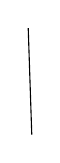
\begin{tikzpicture}[x=1mm,y=1mm]\draw (0,0)--(-0.45,13.5);\end{tikzpicture}}}

% MS 7–9
\uline{\deleted{\unsure{Théorème}}\unsure{Proposition} 3} Le prédérivateur $\mathrm{HOT}$ satisfait aux axiomes Der 1, Der 2 \inserted{(pour mémoire)} et Der $3\,b^{*}$, Der $4'$ \deleted{\unsure{b}}, Der $5'$.

% MS upper right, arrow from Der 2
% slanted
\margin{\uline{pas prouvé} \deleted{\illegible{5}} le ``résultat'' auquel je suis \unsure{``parvenu''} \unsure{est} \unsure{cf. n\textsuperscript{o} 5} p.~165}

% MS right below the proposition
\margin{cf complément prop.~\uline{5} p.~\unsure{167|164}}

% MS left beside Der 3 b
% slanted
\margin{et \unsure{$=$|$\Longleftarrow$} la variante la plus forte Der $3\,b'_2$ de Der 3, cf \unsure{aussi} page suivante.}

% MS left below preceding note
% slanted
\margin{\uline{NB} Pour D $3\,b'_2$, on a utilisé l'axiome L6 ``$W$ est \unsure{dit|clos} \unsure{cf} \unsure{multiplicatif}''. \deleted{et On} voit que $\times_*$ \unsure{la validité} de Der $3\,b'_2$ implique L6 \unsure{bis}, et même la forme plus forte L6 bis, dans cette forme si on exige seulement \unsure{donc} $3\,b''_1$ \unsure{pour} $f_0^*$ pl. fid.}

% MS 10–13
On vient de prouver aussi les variantes \unsure{inférieures} de Der 3, la forme la plus forte de celles-ci (Der $3\,b'_2$) : si $f\in W$, alors $f^*$ induit une \uline{équivalence} de catégories

% MS 14
\[
 f_0^*:\mathrm{HOT}_W^{\mathrm{lc}}(S)\longrightarrow\mathrm{HOT}_W^{\mathrm{lc}}(S').
\]

% MS 15–23
La pleine fidélité du foncteur $f_0^*$ doit résulter de \deleted{Der 3 b} la variante naturelle Der $3\,b''_{\mathrm{coh}}$ de Der 3 b, une fois qu'on aura développé le formalisme des \deleted{\unsure{foncteurs}} Homs internes dans les $\mathrm{HOT}_{\deleted{\unsure{V}}W}(\deleted{\unsure{s}}S)$. Mais \deleted{\unsure{pour}} donner un sens à Der $3\,b''_{\mathrm{coh}}$, on a besoin des foncteurs \uline{cohomologiques}, i.e. de $p_*$ et $p'_*$ \unsure{(au} lieu de $p_!$, $p'_!)$ pour $\mathrm{HOT}$, donc c'est encore prématuré pour l'instant. La construction des $f_*$ et celle des Homs internes \deleted{\unsure{est}}\inserted{\unsure{fera|sera}} d'ailleurs sûrement $\pm$ \unsure{conjointement}.

% archive sheet number: 213
